\chapter{Operator Discovery, Portfolio Control, and Real-World CVRP Studies}
\label{chap:advanced-phases}
\chapterrunning{advanced phases}

The later phases of the project deliberately raise the bar. Instead of asking only whether replay
can help a fixed scaffold, they ask whether the search can discover reusable operators, learn an
interpretable controller over a frozen portfolio, synthesize feasible solver logic on real-world
CVRP instances, or survive explicit matched-budget controls on that same bounded CVRP regime. These
phases distinguish bounded wins from claims the evidence cannot support.

\section{Phase 7: Modular Operator Discovery}
\label{sec:advanced-phase7}

Phase 7 changes the search object from a whole TSP heuristic to a single modular operator. The
official campaign contains twenty paired runs, 800 modular epochs, zero modular generation
fallbacks, zero operator materialization fallbacks, and zero `missing\_build\_operator` failures.
The scientific question, however, is stricter than in the routing replay
phases. A candidate operator is not counted as a discovery unless it survives transplant across
multiple scaffolds, family-level evaluation, ablation, and Pareto-style practicality checks.

Table~\ref{tab:phase7-summary} summarizes the main outcome.

\begin{table}[t]
\centering
\scriptsize
\setlength{\tabcolsep}{3pt}
\begin{tabularx}{\textwidth}{
  >{\raggedright\arraybackslash}p{1.7in}
  Y
}
\toprule
Item & Result \\
\midrule
Best overall condition & full-solver evolution, transfer gap $0.117916$, TSPLIB gap $0.164668$ \\
Best modular condition & modular operator with random replay, transfer gap $0.118833$, TSPLIB gap $0.230474$ \\
Modular evolution vs heuristic-only baseline & transfer delta $-0.001715$, 95\% CI $[-0.003418,0.000085]$; TSPLIB delta $-0.003035$, 95\% CI $[-0.010147,0.000716]$ \\
Modular evolution vs full-solver evolution & TSPLIB delta $+0.067355$, 95\% CI $[0.040498,0.094769]$ in favor of full-solver evolution \\
Validation outcome & no candidate satisfied the conservative surviving-operator rule \\
Rediscovery signal & 56 distinct rediscovery signatures; the most common family was a double-bridge segment-reversal perturbation \\
\bottomrule
\end{tabularx}
\caption[Phase-7 operator-discovery summary]{Phase-7 operator-discovery summary, based on twenty paired offsets. The search
generates recurrent operator families, but no operator survives the full validation pipeline.}
\label{tab:phase7-summary}
\end{table}

The distinction here is between \emph{rediscovery} and \emph{validated discovery}. Rediscovery
means that similar operator families reappear across seeds, which suggests structured attractors in
the search space. Validated discovery requires more: a reusable operator must show positive
transplant evidence, family-level benefit, acceptable runtime behavior, and ablation evidence that
the operator itself matters. No candidate met all of those criteria in the completed campaign.

Phase 7 is therefore a negative result on the retained endpoint, but it remains informative. It
shows that the validation pipeline rejects brittle or scaffold-specific artifacts and prevents an
unsupported reusable-operator claim. Appendix~\ref{sec:appendix-phase7-operator} shows a
representative rediscovered double-bridge perturbation artifact from this phase.

\section{Phase 8: Adaptive Heuristic Portfolio Control}
\label{sec:advanced-phase8}

Phase 8 reframes the problem as algorithm selection. Instead of inventing low-level operators, the
model evolves a bounded and interpretable controller over a frozen portfolio of known TSP
heuristics. This target is more conservative. If phase 7 suggests that reusable low-level
innovation is hard to validate, then a higher-level selection problem may still admit useful
learning.

The completed campaign contains twenty paired runs, eight compared conditions, judge support in
every run, and only three controller-generation errors across the whole replay-aware arm. All
three of those errors occurred in rejected epochs, so no accepted final controller depends on
fallback behavior.

Table~\ref{tab:phase8-summary} gives the key phase-8 comparisons.

\begin{table}[t]
\centering
\scriptsize
\setlength{\tabcolsep}{3pt}
\begin{tabularx}{\textwidth}{
  >{\raggedright\arraybackslash}p{1.7in}
  Y
}
\toprule
Comparison or statistic & Result \\
\midrule
Best held-out TSPLIB condition & best single fixed heuristic, mean gap $0.07226$ \\
Oracle selector vs best fixed heuristic & held-out TSPLIB delta $0.0$; transfer-gap delta $-0.004544$ \\
Supervised selector vs best fixed heuristic & held-out TSPLIB delta $0.0$; transfer-gap delta $0.0$ \\
LLM static selector vs supervised selector & held-out TSPLIB delta $+0.121255$, 95\% CI $[0.099278,0.140226]$ \\
Adaptive controller vs LLM static selector & held-out TSPLIB delta $-0.038118$, 95\% CI $[-0.06868,-0.00707]$ \\
Replay-aware adaptive controller vs no-replay adaptive controller & held-out TSPLIB delta $+0.010114$, 95\% CI $[-0.020641,0.041674]$ \\
Full-solver evolution vs adaptive controller & held-out TSPLIB delta $+0.011853$, 95\% CI $[-0.025032,0.049041]$ \\
\bottomrule
\end{tabularx}
\caption[Phase-8 adaptive-portfolio summary]{Phase-8 adaptive-portfolio summary, based on twenty paired offsets. Lower deltas are
better because the primary endpoint is held-out TSPLIB gap.}
\label{tab:phase8-summary}
\end{table}

The central structural result is the first row of interpretation in
Table~\ref{tab:phase8-summary}: the oracle selector ties the best single fixed heuristic on the
primary held-out TSPLIB endpoint. In algorithm-selection terms, the frozen portfolio has almost no
oracle headroom on that endpoint. If the oracle does not beat the single best fixed heuristic, then
no learned controller should be expected to produce a strong positive selector-regret result there.

This structural constraint explains the mixed phase-8 outcome. The adaptive controller does learn
something
useful relative to a weak one-shot LLM rule baseline, but it does not beat the strongest fixed or
supervised baselines on the primary endpoint. The limitation is not only controller learning. It is
also the lack of complementary headroom in the frozen portfolio being controlled.

\section{Phase 9: Real-World CVRP Solver Evolution}
\label{sec:advanced-phase9}

Phase 9 is the most realistic completed campaign in the dissertation. The search object is now a
bounded whole solver for CVRPLIB Uchoa X instances \cite{uchoa2017}. The solver must return a full
route set, satisfy customer-coverage and vehicle-capacity constraints, and tolerate stronger
validator pressure than the earlier routing scaffolds.

The benchmark split used in the official bounded suite is listed in
Table~\ref{tab:phase9-split}.

\begin{table}[t]
\centering
\scriptsize
\setlength{\tabcolsep}{4pt}
\begin{tabularx}{\textwidth}{Y Y}
\toprule
Training instances & Held-out instances \\
\midrule
X-n101-k25, X-n110-k13, X-n125-k30, X-n134-k13, X-n157-k13, X-n214-k11 & X-n176-k26, X-n190-k8, X-n223-k34, X-n247-k50, X-n275-k28 \\
\bottomrule
\end{tabularx}
\caption[Phase-9 CVRPLIB X split]{Phase-9 bounded CVRPLIB X split, with six training instances and five held-out instances. The
train/held-out separation is fixed before the campaign and is not reopened during solver
evolution.}
\label{tab:phase9-split}
\end{table}

The official phase-9 campaign contains all four conditions in every paired run, judge support
remains enabled throughout, and the accepted solvers do not rely on fallback code or hidden timeout
failures. Across the whole campaign, the solver-evolution arm records 39 accepted epochs out of
160 total epochs, 0 generation fallbacks, 0 accepted errored generations, and full held-out
feasibility in every official run.

Table~\ref{tab:phase9-results} summarizes the main held-out outcomes.

\begin{table}[t]
\centering
\scriptsize
\setlength{\tabcolsep}{3pt}
\begin{tabularx}{\textwidth}{
  >{\raggedright\arraybackslash}p{1.65in}
  c
  c
  Y
}
\toprule
Condition & Held-out feasibility & Mean penalized gap & Reading \\
\midrule
Clarke--Wright savings & 1.0 & 0.073766 & strongest fixed baseline \\
Solver evolution & 1.0 & 0.182231 & bounded positive result, but behind Clarke--Wright \\
Nearest-neighbor constructive & 1.0 & 0.273435 & clearly weaker baseline \\
Regret insertion plus local search & 1.0 & 0.466391 & weakest baseline on the primary endpoint \\
\bottomrule
\end{tabularx}
\caption[Phase-9 held-out CVRP results]{Phase-9 held-out results on bounded real-world CVRP, based on twenty paired runs over the
five held-out X instances. Lower penalized gap is better.}
\label{tab:phase9-results}
\end{table}

The paired comparisons quantify the difference more directly. Solver evolution achieves a held-out penalized gap that
is lower than nearest-neighbor by $0.091204$ penalized-gap units, with a 95\% CI for the paired
delta from $-0.128136$ to $-0.055417$. It also improves on regret-insertion plus local search by
$0.284160$ penalized-gap units, with a 95\% CI from $-0.321769$ to $-0.247706$. Against
Clarke--Wright, however, the sign reverses: solver evolution is higher by $0.108465$
penalized-gap units, with a 95\% CI from $0.071184$ to $0.144731$.

Two additional properties matter for interpretation. First, the solver-evolution arm remains fully
feasible on both train and held-out panels throughout the completed campaign. That means the loop
preserves feasible executable solver updates under validator pressure rather than only generating
low-gap candidates that fail validation.
Second, the resulting solver set is not one repeated artifact. There are sixteen distinct final
solver fingerprints across the twenty official runs, although some no-acceptance runs remain at the
same starting incumbent.

The main limitation is runtime variability. The evolved solvers have mean held-out runtime about
$821.7$ ms, median runtime about $255.2$ ms, and a heavy upper tail above seven seconds in the
worst run-level case. Phase 9 does not support a claim of practical dominance. It is a bounded
real-world result: given only the specification, validator, scorer, and training instances, the
loop can generate feasible held-out solver logic that improves over weaker baselines without
surpassing the strongest fixed heuristic in the benchmark regime.

This runtime profile also clarifies the quality trade-off. The evolved solvers improve the primary
held-out gap relative to the weaker constructive baselines while preserving feasibility, but they do
so with materially less predictable wall-clock cost than the simpler fixed heuristics. In other
words, the phase-9 result is best interpreted as evidence of bounded solution-quality adaptation
under validator pressure, not as a ready-made runtime-efficient replacement for the strongest
classical solver.

Figure~\ref{fig:phase9-diagnostics} makes those boundary conditions explicit at the run level. The
train-versus-held-out scatter shows that the stronger phase-9 runs stay strong off the training
panel rather than collapsing catastrophically out of sample, but the held-out relationship remains
noisy. The runtime panel shows a heavy-tailed cost profile, and the paired delta panels show
why the phase-9 result remains bounded: solver evolution beats the weaker nearest-neighbor
baseline in most matched runs, but it beats Clarke--Wright only in a small minority.

\begin{figure}[p]
\centering
\begin{tikzpicture}
\begin{groupplot}[
  group style={group size=2 by 2, horizontal sep=1.4cm, vertical sep=2.0cm},
  width=0.40\textwidth,
  height=0.20\textheight,
  title style={font=\footnotesize},
  xlabel style={font=\footnotesize},
  ylabel style={font=\footnotesize},
  tick label style={font=\scriptsize},
]
\nextgroupplot[
  title={Train vs held-out gap},
  xlabel={Train penalized gap},
  ylabel={Held-out penalized gap},
  xmin=0.05,
  xmax=0.36,
  ymin=0.05,
  ymax=0.29,
]
\addplot[dashed, black!60] coordinates {(0.05,0.05) (0.36,0.36)};
\addplot[only marks, mark=*, mark size=1.8pt, black] coordinates {
  (0.246296,0.238752) (0.337704,0.273435) (0.197631,0.152817) (0.276613,0.237296)
  (0.216219,0.200191) (0.066394,0.070678) (0.312474,0.268095) (0.337704,0.273435)
  (0.337704,0.273435) (0.068502,0.073101) (0.337704,0.273435) (0.188377,0.206322)
  (0.337704,0.273435) (0.178906,0.171366) (0.063035,0.066878) (0.204197,0.109282)
  (0.066773,0.070771) (0.103492,0.077593) (0.297436,0.263478) (0.067409,0.070818)
};

\nextgroupplot[
  title={Runtime vs quality},
  xlabel={Held-out runtime (ms)},
  ylabel={Held-out penalized gap},
  xmode=log,
  xmin=35,
  xmax=9000,
  ymin=0.05,
  ymax=0.50,
]
\addplot[only marks, mark=*, mark size=1.8pt, black] coordinates {
  (1412.609,0.238752) (138.024,0.273435) (242.935,0.152817) (263.837,0.237296)
  (183.022,0.200191) (7487.227,0.070678) (153.247,0.268095) (136.762,0.273435)
  (137.185,0.273435) (271.581,0.073101) (141.184,0.273435) (295.025,0.206322)
  (138.469,0.273435) (1616.678,0.171366) (1161.820,0.066878) (1462.029,0.109282)
  (246.549,0.070771) (519.746,0.077593) (160.560,0.263478) (265.630,0.070818)
};
\addplot[only marks, mark=square*, mark size=2.2pt, black!70] coordinates {(43.021,0.273435)};
\addplot[only marks, mark=triangle*, mark size=2.3pt, black!55] coordinates {(79.571,0.073766)};
\addplot[only marks, mark=diamond*, mark size=2.3pt, black!35] coordinates {(1473.490,0.466391)};

\nextgroupplot[
  title={Delta vs nearest neighbor},
  xlabel={Paired run index},
  ylabel={Held-out paired delta},
  xmin=0.5,
  xmax=20.5,
  ymin=-0.22,
  ymax=0.02,
  xtick={1,5,10,15,20},
]
\addplot[dashed, black!60] coordinates {(0.5,0) (20.5,0)};
\addplot[only marks, mark=*, mark size=1.8pt, black] coordinates {
  (1,-0.034683) (2,0.000000) (3,-0.120618) (4,-0.036139) (5,-0.073244)
  (6,-0.202757) (7,-0.005340) (8,0.000000) (9,0.000000) (10,-0.200334)
  (11,0.000000) (12,-0.067113) (13,0.000000) (14,-0.102069) (15,-0.206557)
  (16,-0.164153) (17,-0.202664) (18,-0.195842) (19,-0.009957) (20,-0.202617)
};

\nextgroupplot[
  title={Delta vs Clarke--Wright},
  xlabel={Paired run index},
  ylabel={Held-out paired delta},
  xmin=0.5,
  xmax=20.5,
  ymin=-0.02,
  ymax=0.22,
  xtick={1,5,10,15,20},
]
\addplot[dashed, black!60] coordinates {(0.5,0) (20.5,0)};
\addplot[only marks, mark=square*, mark size=1.8pt, black] coordinates {
  (1,0.164986) (2,0.199669) (3,0.079051) (4,0.163530) (5,0.126425)
  (6,-0.003088) (7,0.194329) (8,0.199669) (9,0.199669) (10,-0.000665)
  (11,0.199669) (12,0.132556) (13,0.199669) (14,0.097600) (15,-0.006888)
  (16,0.035516) (17,-0.002995) (18,0.003827) (19,0.189712) (20,-0.002948)
};
\end{groupplot}
\end{tikzpicture}
\caption[Phase-9 diagnostic views]{Diagnostic views for the official phase-9 solver-evolution campaign, using all twenty paired
runs. The upper panels show that good train performance does not guarantee strong held-out
performance and that runtime has a heavy upper tail. The lower panels show the paired held-out
deltas against the two most important baselines. Negative values are better because the endpoint is
lower-is-better penalized gap. In the runtime panel, circular markers denote solver-evolution
runs, while square, triangular, and diamond markers denote nearest-neighbor, Clarke--Wright, and
regret-insertion-plus-local-search baselines.}
\label{fig:phase9-diagnostics}
\end{figure}

Figure~\ref{fig:phase9-phasewise-diagnostics} adds two diagnostics that are not visible in the
final held-out mean alone. First, accepted updates are sparse and spread across the entire
eight-epoch budget rather than concentrated at the start of the run. Second, the instance-level
contrast is uniform in sign: averaged across the twenty official runs, solver evolution beats
nearest-neighbor on all five held-out X instances, but it trails Clarke--Wright on all five.

\begin{figure}[p]
\centering
\begin{minipage}[t]{0.46\textwidth}
\centering
\begin{tikzpicture}
\begin{groupplot}[
  group style={group size=1 by 2, vertical sep=1.75cm},
  width=0.88\textwidth,
  height=0.18\textheight,
  xmin=0.5,
  xmax=8.5,
  xtick={1,2,3,4,5,6,7,8},
  xlabel style={font=\footnotesize},
  ylabel style={font=\footnotesize},
  title style={font=\footnotesize},
  tick label style={font=\scriptsize},
]
\nextgroupplot[
  title={Acceptance rate by epoch},
  ylabel={Share of runs},
  ymin=0,
  ymax=0.45,
]
\addplot+[ybar, draw=black, fill=black!25, bar width=10pt, mark=none] coordinates {
  (1,0.25) (2,0.20) (3,0.30) (4,0.15) (5,0.25) (6,0.30) (7,0.40) (8,0.10)
};

\nextgroupplot[
  title={Median incumbent train gap},
  xlabel={Epoch},
  ylabel={Train penalized gap},
  ymin=0.18,
  ymax=0.35,
]
\addplot+[color=black, mark=*, mark size=1.8pt, mark options={fill=black}] coordinates {
  (1,0.337704) (2,0.337704) (3,0.325089) (4,0.325089)
  (5,0.279921) (6,0.231915) (7,0.210208) (8,0.210208)
};
\end{groupplot}
\end{tikzpicture}
\end{minipage}\hfill
\begin{minipage}[t]{0.46\textwidth}
\centering
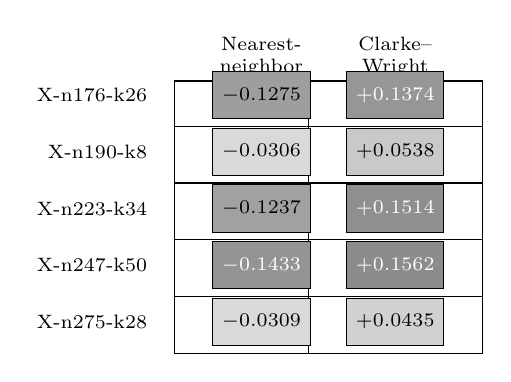
\begin{tikzpicture}[x=1.70cm,y=0.72cm]
\node[font=\scriptsize, align=center] at (1,5.68) {Nearest-\\neighbor};
\node[font=\scriptsize, align=center] at (2,5.68) {Clarke--\\Wright};
\node[font=\scriptsize, anchor=east] at (0.22,5) {X-n176-k26};
\node[font=\scriptsize, anchor=east] at (0.22,4) {X-n190-k8};
\node[font=\scriptsize, anchor=east] at (0.22,3) {X-n223-k34};
\node[font=\scriptsize, anchor=east] at (0.22,2) {X-n247-k50};
\node[font=\scriptsize, anchor=east] at (0.22,1) {X-n275-k28};
\draw[black] (0.35,0.45) rectangle (2.65,5.25);
\draw[black] (1.35,0.45) -- (1.35,5.25);
\foreach \y in {1.45,2.45,3.45,4.45} {
  \draw[black] (0.35,\y) -- (2.65,\y);
}
\node[draw=black, fill=black!38, minimum width=1.0cm, minimum height=0.6cm, font=\scriptsize] at (1,5) {$-0.1275$};
\node[draw=black, fill=black!41, minimum width=1.0cm, minimum height=0.6cm, font=\scriptsize, text=white] at (2,5) {$+0.1374$};
\node[draw=black, fill=black!15, minimum width=1.0cm, minimum height=0.6cm, font=\scriptsize] at (1,4) {$-0.0306$};
\node[draw=black, fill=black!21, minimum width=1.0cm, minimum height=0.6cm, font=\scriptsize] at (2,4) {$+0.0538$};
\node[draw=black, fill=black!37, minimum width=1.0cm, minimum height=0.6cm, font=\scriptsize] at (1,3) {$-0.1237$};
\node[draw=black, fill=black!44, minimum width=1.0cm, minimum height=0.6cm, font=\scriptsize, text=white] at (2,3) {$+0.1514$};
\node[draw=black, fill=black!42, minimum width=1.0cm, minimum height=0.6cm, font=\scriptsize, text=white] at (1,2) {$-0.1433$};
\node[draw=black, fill=black!45, minimum width=1.0cm, minimum height=0.6cm, font=\scriptsize, text=white] at (2,2) {$+0.1562$};
\node[draw=black, fill=black!15, minimum width=1.0cm, minimum height=0.6cm, font=\scriptsize] at (1,1) {$-0.0309$};
\node[draw=black, fill=black!18, minimum width=1.0cm, minimum height=0.6cm, font=\scriptsize] at (2,1) {$+0.0435$};
\end{tikzpicture}
\end{minipage}
\caption[Additional phase-9 diagnostics]{Additional diagnostics for the official phase-9 solver-evolution campaign. The left panels use all
twenty official runs and track the accepted-update rate by epoch together with the median incumbent
train penalized gap, starting from the shared nearest-neighbor constructive incumbent. The right
panel aggregates the five held-out X instances across the same twenty runs. Solver evolution beats
nearest-neighbor on every held-out instance, but it trails Clarke--Wright on every held-out
instance. Darker cells mark larger absolute differences, and negative values favor solver
evolution.}
\label{fig:phase9-phasewise-diagnostics}
\end{figure}

Appendix~\ref{sec:appendix-phase9-solver} shows a representative accepted phase-9 solver fragment,
and Appendix~\ref{sec:appendix-phase9-failure} records a representative validator rejection. Those
artifacts help explain both sides of the result: the loop can preserve feasible route-improvement
logic, but validator pressure still filters out many large or syntactically salvaged candidates.

\section{Phase 9 Closeout: Budget-Control CVRP Study}
\label{sec:advanced-phase9-closeout}

The original phase-9 campaign established that bounded solver evolution on real-world CVRP is
feasible and stronger than the weakest fixed baselines, but it left one mechanism question open:
was replay helping because it preserved useful incumbent structure, or simply because the loop was
allowed to spend more candidate budget than a direct generation baseline? The closeout keeps the
same bounded CVRPLIB X split, validator, and held-out endpoint, then introduces matched learned
controls to answer that narrower question directly.

The official closeout campaign contains all six conditions in every paired run, judge support
remains enabled throughout, and the three learned closeout arms record zero generation fallbacks
and zero generation errors. Replay-aware solver evolution is also the only learned arm with full
held-out feasibility in all twenty official runs. The budget-matched no-replay arm remains feasible
in only three runs, and the direct-generate-plus-one-repair arm remains feasible in only five.

Table~\ref{tab:phase9-closeout-results} summarizes the held-out outcome.

\begin{table}[t]
\centering
\scriptsize
\setlength{\tabcolsep}{3pt}
\begin{tabularx}{\textwidth}{
  >{\raggedright\arraybackslash}p{1.7in}
  c
  c
  Y
}
\toprule
Condition & Held-out feasibility & Mean penalized gap & Reading \\
\midrule
Clarke--Wright savings & 1.0 & 0.073766 & strongest fixed baseline, unchanged from the original phase-9 suite \\
Replay solver evolution & 1.0 & 0.171114 & only learned arm with full held-out feasibility under the closeout controls \\
Nearest-neighbor constructive & 1.0 & 0.273435 & weaker fixed baseline retained for continuity with phase 9 \\
Regret insertion plus local search & 1.0 & 0.466391 & weakest fixed baseline on the primary endpoint \\
Budget-matched no replay & 0.15 & 2.932746 & memoryless learned control with the same overall candidate budget \\
Direct generate plus one repair & 0.25 & 5.286402 & bounded direct-synthesis control with one scripted repair step \\
\bottomrule
\end{tabularx}
\caption[Phase-9 closeout held-out CVRP results]{Held-out results for the official phase-9 closeout campaign, based on twenty paired runs over
the same five held-out X instances used in the original phase-9 suite. Lower penalized gap is
better.}
\label{tab:phase9-closeout-results}
\end{table}

The paired closeout comparisons quantify the mechanism difference more directly. Replay-aware solver evolution achieves a
held-out penalized gap that is lower than the budget-matched no-replay control by $2.761632$
penalized-gap units, with a 95\% CI for the paired delta from $-3.369777$ to $-2.201586$. It also
beats the direct-generate-plus-one-repair control by $5.115288$ penalized-gap units, with a 95\%
CI from $-7.451608$ to $-2.946446$. Against Clarke--Wright, however, the sign remains
unfavorable: replay-aware solver evolution is higher by $0.097348$ penalized-gap units, with a
95\% CI from $0.055994$ to $0.138558$.

The closeout addresses the mechanism question because the weaker learned arms fail in different
ways. The
budget-matched no-replay arm accepts more epochs than replay-aware solver evolution, yet it often
produces code changes that do not preserve held-out feasibility. The bounded direct control
occasionally produces a strong feasible solver, but it is unstable and usually collapses on the
same held-out panel. These contrasts indicate that replay contributes more than extra candidate
count alone: in this bounded regime it stabilizes the search around an incumbent well enough to
dominate both learned controls, even though it still does not beat the strongest fixed
Clarke--Wright baseline.

\section{Interpretive Pattern Across the Later Phases}
\label{sec:advanced-interpretation}

Phases 7 through the phase-9 closeout share a common pattern. Once the search object or validator
becomes more demanding, the loop continues to produce executable diversity, but the surviving
positive claims become narrower.

Phase 7 shows rediscovery without validated reusable operator discovery. Phase 8 shows adaptive
learning over a weak one-shot LLM baseline, but not over the strongest fixed or supervised
selectors when selector headroom is absent. Phase 9 shows feasible real-world solver evolution
that beats weak baselines, but not the best fixed baseline. The phase-9 closeout shows that
replay-aware incumbent-preserving search has a measurable advantage over matched learned controls,
yet still not enough to displace the strongest fixed classical baseline.

Taken as a whole, these later phases motivate the capability-bounded interpretation adopted in the
dissertation. The retained evidence still includes non-zero held-out improvement under some
conditions, yet the later phases repeatedly block the stronger claim that the system is already
discovering dominant general-purpose optimization methods.
